% !TeX root = 机器人学学习笔记.tex
% ============================================================
%  位形空间
%  内容依据 Lynch & Park《Modern Robotics》第 2 章
%  记号约定：向量（含希腊字母）用 \boldsymbol{}
% ============================================================

\begin{definition}[位形（\textit{configuration}）]
	机器人所有点位置的坐标参数化描述。因为机器人的连杆都是刚性的，且有固定的形状，所以描述机器人的位形只需要几个数即可。
\end{definition}

\begin{definition}[自由度（\textit{dof}）]
	描述一个机器人位形所需的最小实坐标的个数。
\end{definition}

\section{自由度}

系统自由度=（点的自由度之和）$-$（独立约束数）=（变量数）$-$（独立约束方程数）

而对于由构件组成的机器人系统，自由度=（构件的自由度之和）$-$（独立约束数）

对于机器人系统，自由度来自于构件和关节，所以确定机器人的自由度只需要统计构件和关节的数量即可。于是有格鲁布勒公式。

\textbf{格鲁布勒公式}（\textit{Grübler's Formula}）
\begin{equation}
	\label{eq:自由度:格鲁布勒公式}
	\mathrm{dof}=m(N-1)-\sum_{i=1}^{J}c_{i}=m(N-1)-\sum_{i=1}^{J}(m-f_{i})=m(N-1-J)+\sum_{i=1}^{J}f_{i}
\end{equation}
\begin{itemize}
	\item $N$：包含大地构件的总构件数目；
	\item $m$：自由单刚体的自由度（平面 $m=3$，空间 $m=6$）；
	\item $J$：机器人关节的个数；
	\item $f_{i}$：关节 $i$ 提供的自由度数量；
	\item $c_{i}$：关节 $i$ 提供的约束数。
\end{itemize}

常见关节的自由度和约束数如下：
\begin{table}[H]
	\centering
	\caption{常见关节的自由度和约束数}
	\label{tab:自由度:常见关节}
	\begin{tabular}{lcc}
		\hline
		关节类型 & 自由度数 dof & 提供约束个数 $c_{i}$ \\
		\hline
		转动关节（R） & 1 & 5 \\
		直线关节（P） & 1 & 5 \\
		螺旋关节（H） & 1 & 5 \\
		圆柱关节（C） & 2 & 4 \\
		虎克铰或万向节（U） & 2 & 4 \\
		球铰（S） & 3 & 3 \\
		\hline
	\end{tabular}
\end{table}

自由度就是位形空间的维数。

\section{位形空间的拓扑结构与表示法}

上面讨论了位形空间的维数——自由度。下面关注位形空间的形状，即位形空间的拓扑结构。

\begin{definition}[拓扑等效（\textit{topologically equivalent}）]
	若一个空间可以连续变形成另一个空间，且无需进行切割和粘合，我们称这两个空间是拓扑等效的。
\end{definition}

拓扑学上互不相同的一维空间包括圆、直线以及直线上的闭区间。
\begin{itemize}
	\item 圆在数学上记为 $\mathbb{S}$ 或 $\mathbb{S}^{1}$，即一维球面；
	\item 直线在数学上记为 $\mathbb{E}$ 或 $\mathbb{E}^{1}$，即一维的欧氏空间（平坦空间）；
	\item 直线上的闭区间在数学上记为 $[a,b]\subset\mathbb{R}^{1}$。
\end{itemize}

\textbf{注意}：直线上的开区间和直线拓扑等效，因为可以连续变化成一条直线。

在更高维空间中，$\mathbb{R}^{n}$ 表示 $n$ 维欧几里得空间，而 $\mathbb{S}^{n}$ 表示 $n$ 维球面在 $(n+1)$ 维空间中的曲面。

\textbf{注意}：空间的拓扑结构是该空间本身的一个基本属性，且与我们如何选择坐标来表示空间中的点无关。

某些位形空间可表示为两个或多个低维空间的笛卡尔积；也就是说，此类位形空间中的点可表示为这些低维空间中点的表示方式的并集。例如
\begin{itemize}
	\item 平面内刚体的位形空间可写为 $\mathbb{R}^{2}\times\mathbb{S}^{1}$，因为其位形可以表示为坐标与角度 $\theta$ 的拼接。
	\item PR 机械臂的位形空间可写为 $\mathbb{R}^{1}\times\mathbb{S}^{1}$。（在表述位形空间的拓扑时，我们有时会忽略关节限位，即关节行程的边界；若考虑关节限位，则位形空间是直线上两个闭区间的笛卡儿积。）
\end{itemize}

为了进行计算，我们必须为位形空间建立一个数值表示法，该表示法由一组实数构成。

\textbf{显式参数化}：选择 $n$ 个坐标（或参数）来表示 $n$ 维空间。

显式参数化可能会面临奇异的问题。比如用经纬度坐标系对球体的表示方法在南北极附近的位置，即使迈出极小的一步也可能导致坐标值发生巨大的变化。北极与南极是该表示方法中的奇点。

奇点的存在源于球体与平面在拓扑结构上并不相同——具体而言，用于表示球体的两个实数空间（即经纬度）与平面的实数空间并不相同。这些奇点的位置与球体本身（其在任何位置看起来都相同）并无直接关系，而完全取决于所采用的表示方式。

为了解决奇点的问题，\textit{Lynch} 给出了两种解决方法：
\begin{itemize}
	\item 在空间中使用多个坐标图，其中每个坐标图均为一个显式参数化映射，仅覆盖空间中的某一部分；且在每个坐标图内均不存在奇点。当配置表示法在某个坐标图（例如北极或南极）处趋近于奇点时，只需切换至另一个坐标图——在该坐标图中，北极与南极均远离奇点。
	\begin{itemize}
		\item 优点：坐标图册的表示采用最少数量的图册。
		\item 缺点：需要除了坐标图册外的额外的记录来实现坐标图间的转换和奇异点的规避。
	\end{itemize}
	\item \textbf{隐式参数化}：将要表示的 $n$ 维位形空间嵌入一个高于 $n$ 维的位形空间中。如用 $x^{2}+y^{2}+z^{2}=1$ 来表示一个球面。
	\begin{itemize}
		\item 缺点：参数多了。
		\item 优点：无奇异且在闭环结构中易于找出隐式表达——即有满足闭环方程的关节坐标集合。
	\end{itemize}
\end{itemize}

\section{位形与速度约束}

对于图~\ref{fig:四连杆机构} 这样的一个四连杆机构，采用隐式表达可以用下面三个方程表示出这个机构的位形：
\begin{figure}[htbp]
	\centering
	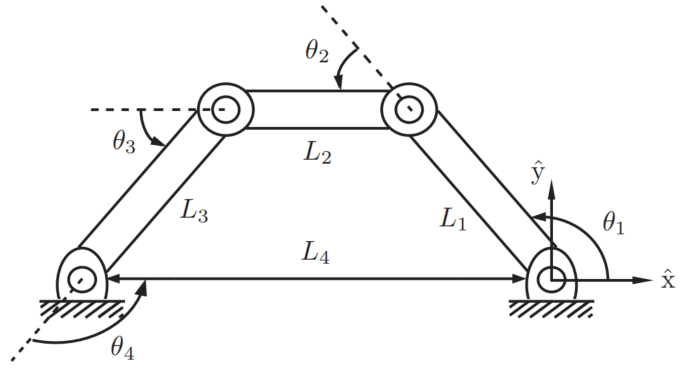
\includegraphics[width=0.5\textwidth]{Figure/四连杆机构.png}
	\caption{四连杆机构}
	\label{fig:四连杆机构}
\end{figure}
\begin{equation}
	\label{eq:位形与速度约束:四连杆闭环方程}
	\begin{aligned}
		L_{1}\cos\theta_{1}+L_{2}\cos(\theta_{1}+\theta_{2})+\cdots+L_{4}\cos(\theta_{1}+\cdots+\theta_{4})&=0,\\
		L_{1}\sin\theta_{1}+L_{2}\sin(\theta_{1}+\theta_{2})+\cdots+L_{4}\sin(\theta_{1}+\cdots+\theta_{4})&=0,\\
		\theta_{1}+\theta_{2}+\theta_{3}+\theta_{4}-2\pi&=0.
	\end{aligned}
\end{equation}
上述方程被称为\textbf{闭环方程}（\textit{loop-closure equations}）。上述方程组的解对应四维空间关节中的一维曲线，并构成位形空间。

对于一个一般的含有一个或多个闭环的机器人系统，位形空间可以被隐式表示成
\begin{equation}
	\label{eq:位形与速度约束:位形向量}
	\boldsymbol{\theta}=\begin{bmatrix}
		\theta_{1}\\
		\vdots\\
		\theta_{n}
	\end{bmatrix}
\end{equation}
闭环方程可以被表示成
\begin{equation}
	\label{eq:位形与速度约束:闭环方程向量形式}
	\boldsymbol{g}(\boldsymbol{\theta})=\begin{bmatrix}
		g_{1}(\theta_{1},\ldots,\theta_{n})\\
		\vdots\\
		g_{k}(\theta_{1},\ldots,\theta_{n})
	\end{bmatrix}=\boldsymbol{0}
\end{equation}
这样的约束显然是完整约束，能有效减少位形空间的维数。这样的话，位形空间就可以看成嵌入 $n$ 维空间中的 $n-k$ 维曲面。

对方程 $\boldsymbol{g}(\boldsymbol{\theta}(t))=\boldsymbol{0}$ 两边对时间进行微分，得：
\begin{equation}
	\label{eq:位形与速度约束:时间导数}
	\begin{bmatrix}
		\frac{\partial g_{1}}{\partial \theta_{1}}(\boldsymbol{\theta})\dot{\theta}_{1}+\cdots+\frac{\partial g_{1}}{\partial \theta_{n}}(\boldsymbol{\theta})\dot{\theta}_{n}\\
		\vdots\\
		\frac{\partial g_{k}}{\partial \theta_{1}}(\boldsymbol{\theta})\dot{\theta}_{1}+\cdots+\frac{\partial g_{k}}{\partial \theta_{n}}(\boldsymbol{\theta})\dot{\theta}_{n}
	\end{bmatrix}=\boldsymbol{0}.
\end{equation}
也可进一步写成：
\begin{equation}
	\label{eq:位形与速度约束:雅可比形式}
	\begin{bmatrix}
		\frac{\partial g_{1}}{\partial \theta_{1}}(\boldsymbol{\theta}) & \cdots & \frac{\partial g_{1}}{\partial \theta_{n}}(\boldsymbol{\theta})\\
		\vdots & \ddots & \vdots\\
		\frac{\partial g_{k}}{\partial \theta_{1}}(\boldsymbol{\theta}) & \cdots & \frac{\partial g_{k}}{\partial \theta_{n}}(\boldsymbol{\theta})
	\end{bmatrix}
	\begin{bmatrix}
		\dot{\theta}_{1}\\
		\vdots\\
		\dot{\theta}_{n}
	\end{bmatrix}=\boldsymbol{0}
\end{equation}
简记为：
\begin{equation}
	\label{eq:位形与速度约束:速度约束}
	\frac{\partial \boldsymbol{g}}{\partial \boldsymbol{\theta}}(\boldsymbol{\theta})\dot{\boldsymbol{\theta}}=\boldsymbol{0}
\end{equation}
进一步简记为：
\begin{equation}
	\label{eq:位形与速度约束:速度约束矩阵形式}
	A(\boldsymbol{\theta})\dot{\boldsymbol{\theta}}=\boldsymbol{0}
\end{equation}
矩阵 $A(\boldsymbol{\theta})\in\mathbb{R}^{k\times n}$。这个形式的速度约束称为\textbf{Pfaffian 约束}。

值得注意的是，Pfaffian 约束不一定是完整约束，因为 $A(\boldsymbol{\theta})$ 未必可积。

\section{任务空间和工作空间}

\begin{definition}[任务空间]
	机器人的任务能够自然表达的空间。
\end{definition}

\begin{definition}[工作空间]
	机器人的末端执行器能够到达位形的空间，取决于机器人的结构。
\end{definition}
